\documentclass[tikz,border=8pt]{standalone}
% Shared look for every TikZ diagram. Load with \input{../../tools/tikz-style.tex}
\usepackage[T1]{fontenc}
\usepackage{lmodern}
\renewcommand{\sfdefault}{lmr}  % diagrams use the same serif as the text
\usetikzlibrary{arrows.meta, positioning, shapes.geometric, calc, fit, backgrounds}
\definecolor{cblue}{HTML}{4C78A8}
\definecolor{corange}{HTML}{F58518}
\definecolor{cgreen}{HTML}{54A24B}
\definecolor{cred}{HTML}{E45756}
\definecolor{cpurple}{HTML}{B279A2}
\definecolor{cgrey}{HTML}{6B6B6B}
\tikzset{
  every picture/.style={font=\sffamily, line width=1.2pt},
  box/.style={draw=#1, fill=#1!12, rounded corners=4pt, align=center, inner sep=7pt, minimum height=1.1cm},
  box/.default=cgrey,
  arrow/.style={-{Stealth[length=3mm]}, draw=cgrey, line width=1.4pt},
  title/.style={font=\sffamily\bfseries\Large},
  note/.style={font=\sffamily\small, text=cgrey, align=center},
}
\AtBeginDocument{\hyphenpenalty=10000 \exhyphenpenalty=10000}

\begin{document}
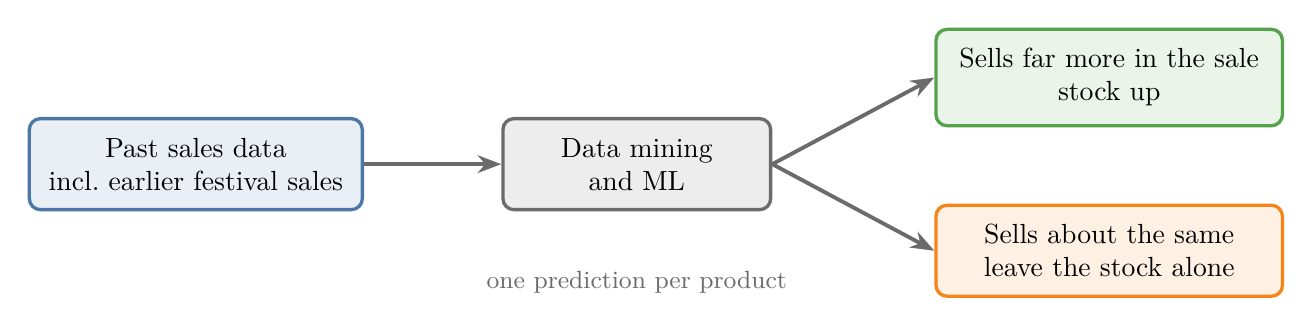
\begin{tikzpicture}
  \node[box=cblue, minimum width=3.8cm] (d) at (0,0) {Past sales data\\incl.\ earlier festival sales};
  \node[box=cgrey, minimum width=3.4cm] (m) at (5.6,0) {Data mining\\and ML};
  \node[box=cgreen, minimum width=4.4cm] (up) at (11.6,1.1) {Sells far more in the sale\\stock up};
  \node[box=corange, minimum width=4.4cm] (no) at (11.6,-1.1) {Sells about the same\\leave the stock alone};
  \draw[arrow] (d) -- (m);
  \draw[arrow] (m.east) -- (up.west);
  \draw[arrow] (m.east) -- (no.west);
  \node[note] at (5.6,-1.5) {one prediction per product};
\end{tikzpicture}
\end{document}
